\documentclass[a4paper,reqno]{amsart}
\usepackage{amsmath}
\usepackage{amssymb}
\usepackage{tikz}
\usetikzlibrary{calc}
\usepackage{tikz-cd}

\newcommand{\Z}{\mathbb{Z}}

\begin{document}

	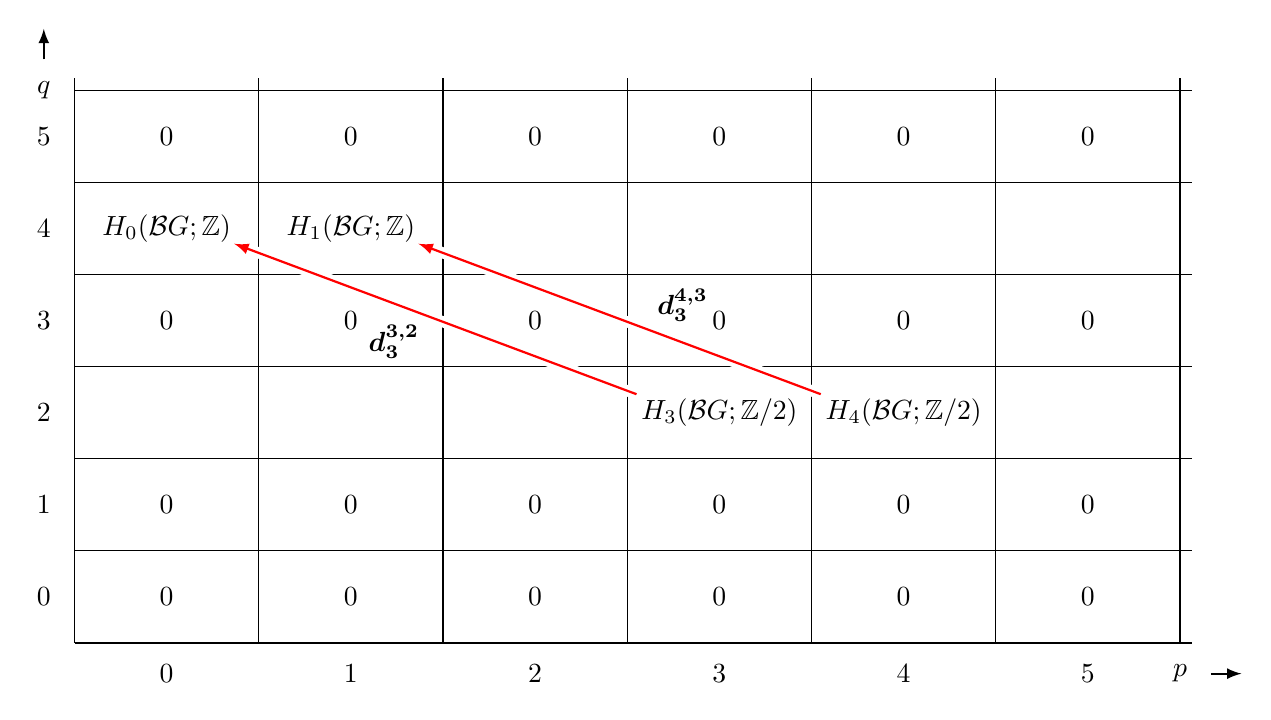
\begin{tikzpicture}[scale=0.78,on top/.style={preaction={draw=white,-,line width=#1}},
		on top/.default=4pt]
		
		\draw[step=3,black] (0,0) grid (18.2, 9.2); %Grid
		
		\draw (0,1.5) -- (18.2,1.5); %Extra horizontal rules
		\draw (0,4.5) -- (18.2,4.5);
		\draw (0,7.5) -- (18.2,7.5);
		
		\node at (1.5,-0.5) {$0$}; %Horizontal labels
		\node at (4.5,-0.5) {$1$};
		\node at (7.5,-0.5) {$2$};
		\node at (10.5,-0.5) {$3$};
		\node at (13.5,-0.5) {$4$};
		\node at (16.5,-0.5) {$5$};
		\node at (18,-0.5) {$p$};
	
		\node at (-0.5,0.75) {$0$}; %Vertical labels
		\node at (-0.5,2.25) {$1$};
		\node at (-0.5,3.75) {$2$};
		\node at (-0.5,5.25) {$3$};
		\node at (-0.5,6.75) {$4$};
		\node at (-0.5,8.25) {$5$};
		\node at (-0.5,9) {$q$};

		\node at (1.5,0.75) {$0$}; % Row 0
		\node at (4.5,0.75) {$0$};
		\node at (7.5,0.75) {$0$};
		\node at (10.5,0.75) {$0$};
		\node at (13.5,0.75) {$0$};
		\node at (16.5,0.75) {$0$};
		
		\node at (1.5,2.25) {$0$}; % Row 1
		\node at (4.5,2.25) {$0$};
		\node at (7.5,2.25) {$0$};
		\node at (10.5,2.25) {$0$};
		\node at (13.5,2.25) {$0$};
		\node at (16.5,2.25) {$0$};
		
		\node at (10.5,3.75) {$H_3(\mathcal{B}G;\Z/2)$}; % Row 2
		\node at (13.5,3.75) {$H_4(\mathcal{B}G;\Z/2)$}; 
		
		\node at (1.5,5.25) {$0$}; % Row 3
		\node at (4.5,5.25) {$0$};
		\node at (7.5,5.25) {$0$};
		\node at (10.5,5.25) {$0$};
		\node at (13.5,5.25) {$0$};
		\node at (16.5,5.25) {$0$};
		
		\node at (1.5,6.75) {$H_0(\mathcal{B}G;\Z)$}; % Row 4
		\node at (4.5,6.75) {$H_1(\mathcal{B}G;\Z)$};
		
		\node at (1.5,8.25) {$0$}; % Row 5
		\node at (4.5,8.25) {$0$};
		\node at (7.5,8.25) {$0$};
		\node at (10.5,8.25) {$0$};
		\node at (13.5,8.25) {$0$};
		\node at (16.5,8.25) {$0$};
				
		\draw [thick, -latex, red](9.15,4.05) [on top]-- (2.6,6.5);
		\draw [thick, -latex, red](12.15,4.05) [on top] -- (5.6,6.5);
		\node at (5.2,4.9) {$\boldsymbol{d_3^{3,2}}$};
		\node at (9.9,5.5) {$\boldsymbol{d_3^{4,3}}$};
		\draw [thick, -latex] (18.5,-0.5) -- (19,-0.5);
		\draw [thick, -latex] (-0.5, 9.5) -- (-0.5,10);
	\end{tikzpicture}

\end{document}